% [原文 p.203]
此结果可看作 de Rham 定理（见前文）的同伦论类比。
利用 (2.66)，现在可以构造所需的同伦不变积分。给定任意光滑映射 $F:S^{q+1}\times\R\to M^n$，我们得到自然同态
\[
  \hat F:C_q(A)\to\Lambda^*(S^{q+1}\times\R),\qquad A=\Lambda^*(M^n),
\]
它与 $d$ 交换：只需在 $C^0_q=A=\Lambda^*(M^n)$ 上令 $\hat F=F^*$，再利用 $S^{q+1}\times\R$ 上次数 $\le q$ 的闭形式都恰当这一事实延拓即可。若 $z$ 是 $H^{q+1}(C_q(A))$ 中任一元素，由闭上链 $\tilde z$ 代表，则 $\hat F(\tilde z)$ 是 $S^{q+1}\times\R$ 上的 $(q+1)$-形式，满足 $d\hat F(\tilde z)=0$。现在定义积分为
\begin{equation}
  H(t)=H(f_t,\tilde z)=\int_{S^{q+1}\times\{t\}}\hat F(\tilde z), \tag{2.67}
\end{equation}
其中
\[
  f_t=\hat F|_{S^{q+1}\times\{t\}}.
\]
由于形式 $\hat F(\tilde z)$ 闭，故 $dH/dt=0$；积分 (2.67) 的同伦不变性由此立即推出。在此背景下「刚性」的定义与考察则要复杂一些。

\section[光滑流形与同伦论。 配边。 Hirzebruch 公式]{光滑流形与同伦论。标架流形。配边。Thom 空间。Hirzebruch 公式。球面同伦群阶的估计。Milnor 的例子。配边的整性性质}
\takeaway{本节用流形几何直接触及映射的同伦类：依次引入标架流形与配边、Thom 空间与 Thom 同态，由此得到 Hirzebruch 公式、球面同伦群阶的估计、Milnor 的怪异球面例子，以及配边的整性性质。核心手法是把「用流形实现同调类」与「沿纤维积分」对偶起来。}

本节先考察一些基于流形几何的想法，借初等手段获取关于流形映射的同伦类的某些信息（情形不同于第 3 章所考察的那些——那里的同伦群因初等理由已知为平凡）。在进一步发展中，这些几何想法与第 3 章末尾所述的代数技术相结合。
我们提醒读者：对光滑流形，任意连续映射与同伦都可被光滑映射任意逼近，且在原映射本已光滑处与之重合；因此我们总是假定流形的映射与同伦在需要时属于 $C^\infty$ 类。

% [原文 p.204]
\begin{figure}[htbp]
  \centering
  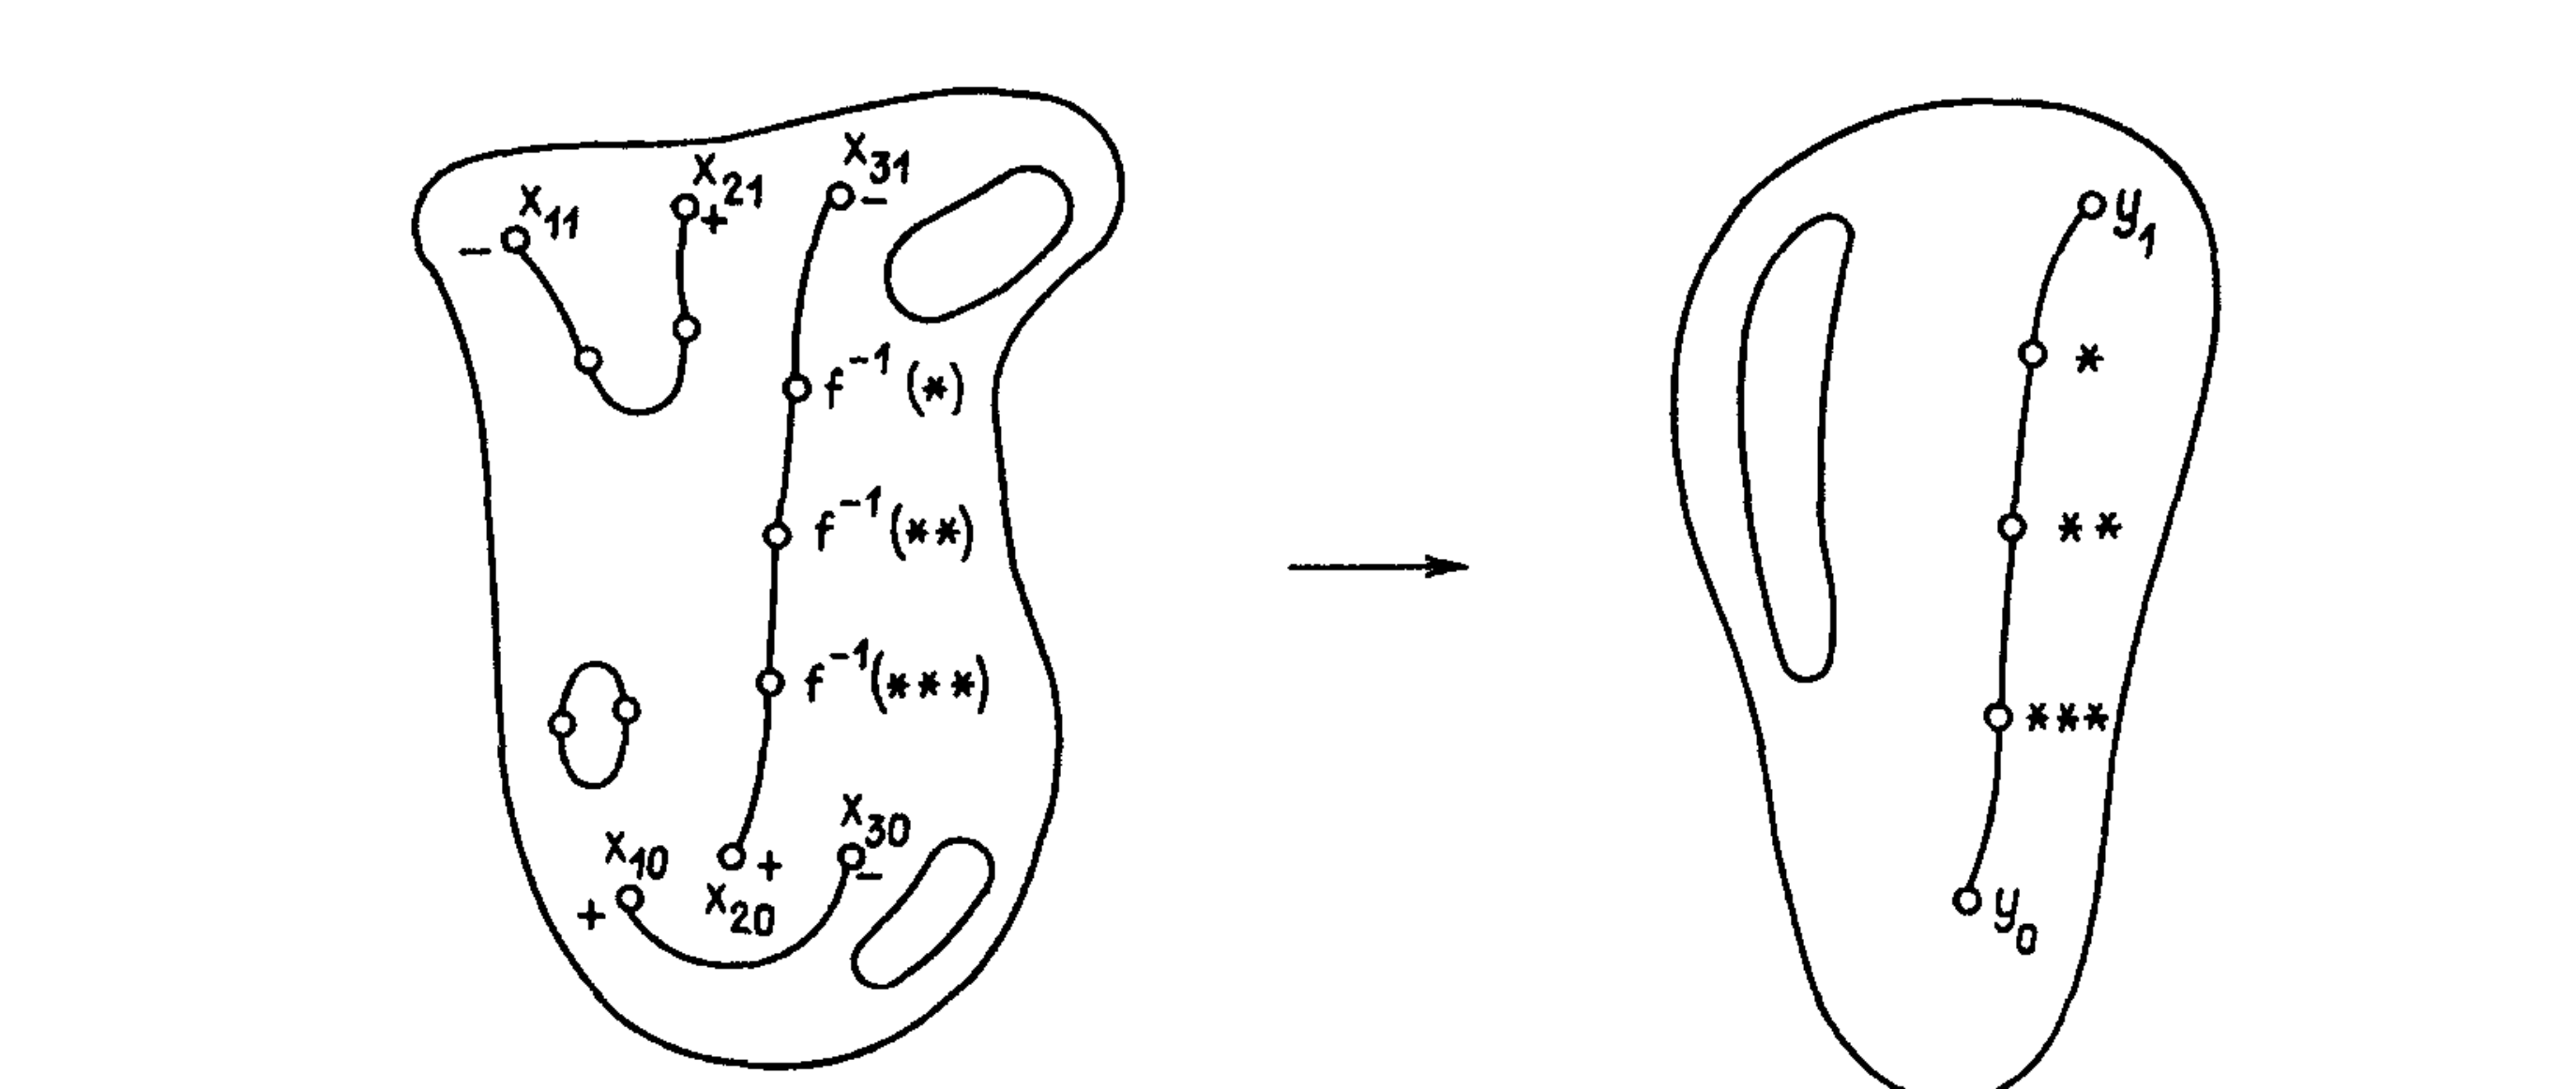
\includegraphics[width=0.92\textwidth]{figures/fig4_15.png}
  \figtitle{4.15}{映射 $f:M^n\to N^n$ 的度：左侧曲面上的原像点成对出现。}
\end{figure}

最简单的同伦不变量是闭可定向同维流形之间映射的\emph{度}（degree）：
\[
  f:M^n\to N^n,
\]
它定义如下：取 $N^n$ 中一个一般位置的点 $y$（即「正则」点）；于是 $f$ 的 Jacobi 矩阵 $J_f$ 在完全原像 $f^{-1}(y)=\{x_1,\dots,x_k\}$ 的每一点处都非零。我们定义
\begin{equation}
  \deg f=\sum_{j=1}^k\sgn J_f(x_j). \tag{3.1}
\end{equation}
（图 4.15 可用来图示「$f$ 的度与 $N^n$ 中正则点 $y$ 的选取无关」这一验证，这里假定 $M^n$ 与 $N^n$ 连通。图 4.16、4.17 例示这一概念。）
\begin{figure}[htbp]
  \centering
  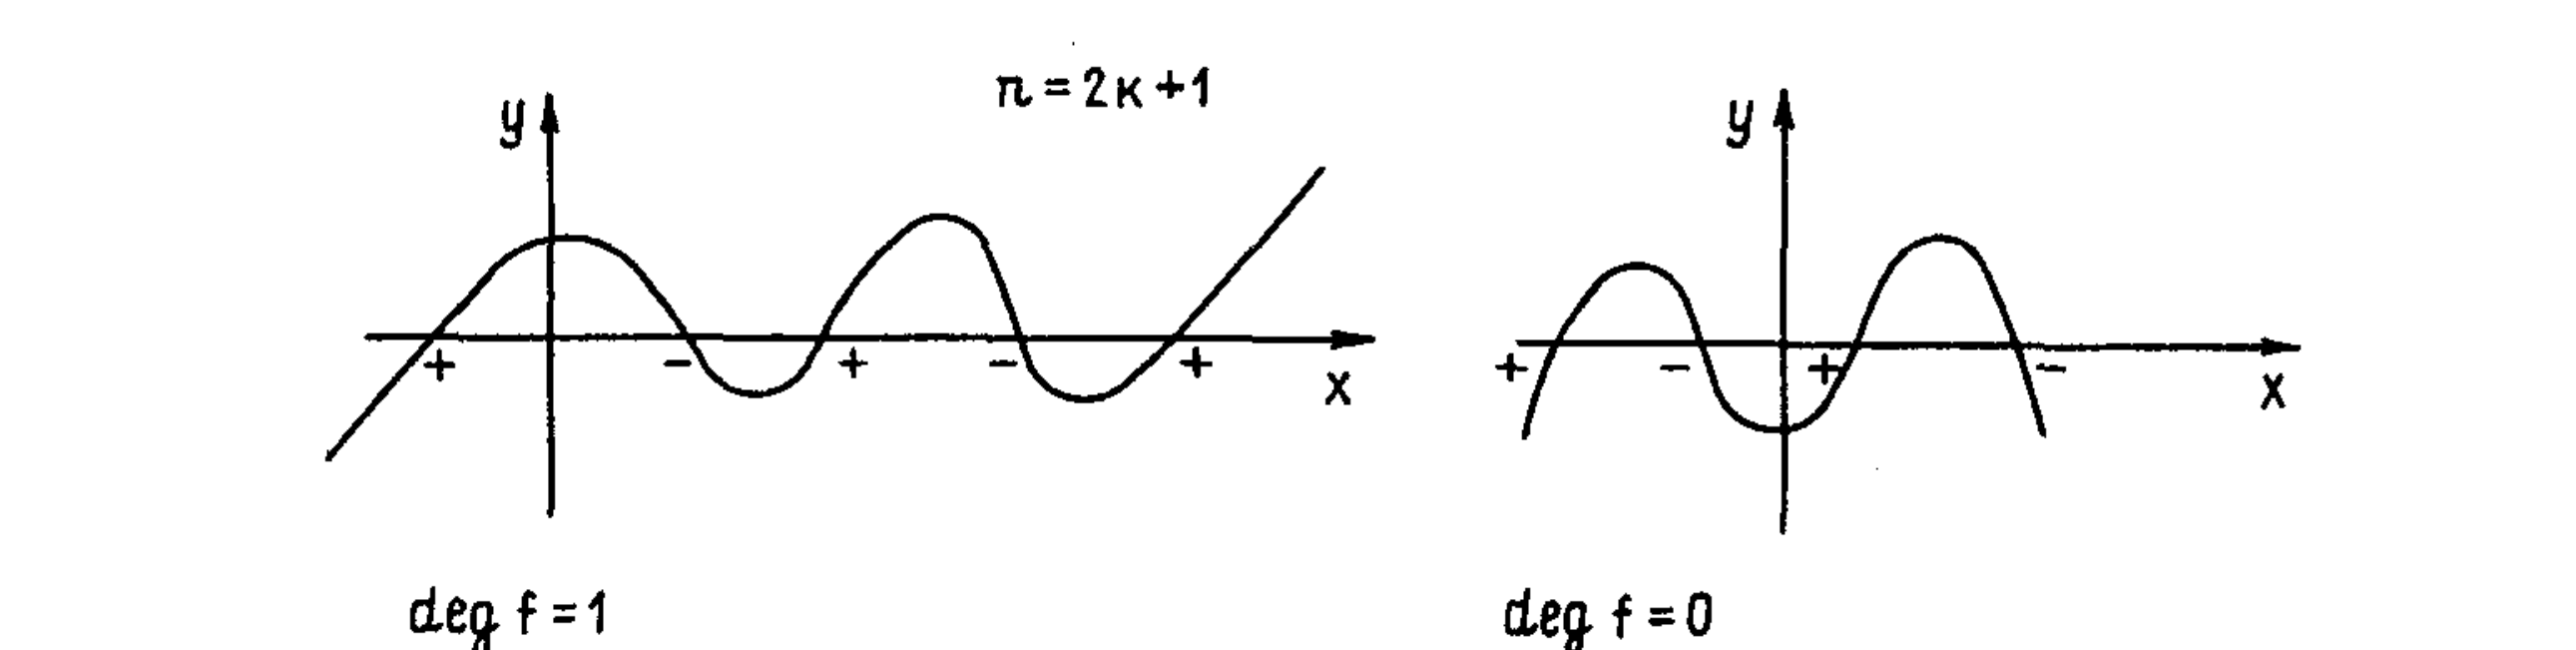
\includegraphics[width=0.86\textwidth]{figures/fig4_16.png}
  \figtitle{4.16}{一维情形：函数图像的符号交替给出度 $1$ 与度 $0$。}
\end{figure}

映射度的定义 (3.1) 也适用于以下情形：

% [原文 p.205]
\para{a)} 映射 $f:(M^n,W^{n-1})\to(N^n,V^{n-1})$，其中 $\partial M^n=W^{n-1}$，$\partial N^n=V^{n-1}$，且把 $M^n$ 的边界 $W^{n-1}$ 映入 $N^n$ 的边界 $V^{n-1}$。此时 $f$ 限制在边界 $W^{n-1}$ 上的度，等于它在 $M^n$ 内部上的度。（于是若 $f$ 在边界之间给出微分同胚，则作为内部之间的映射，必有 $\deg f=\pm1$。）
\begin{figure}[htbp]
  \centering
  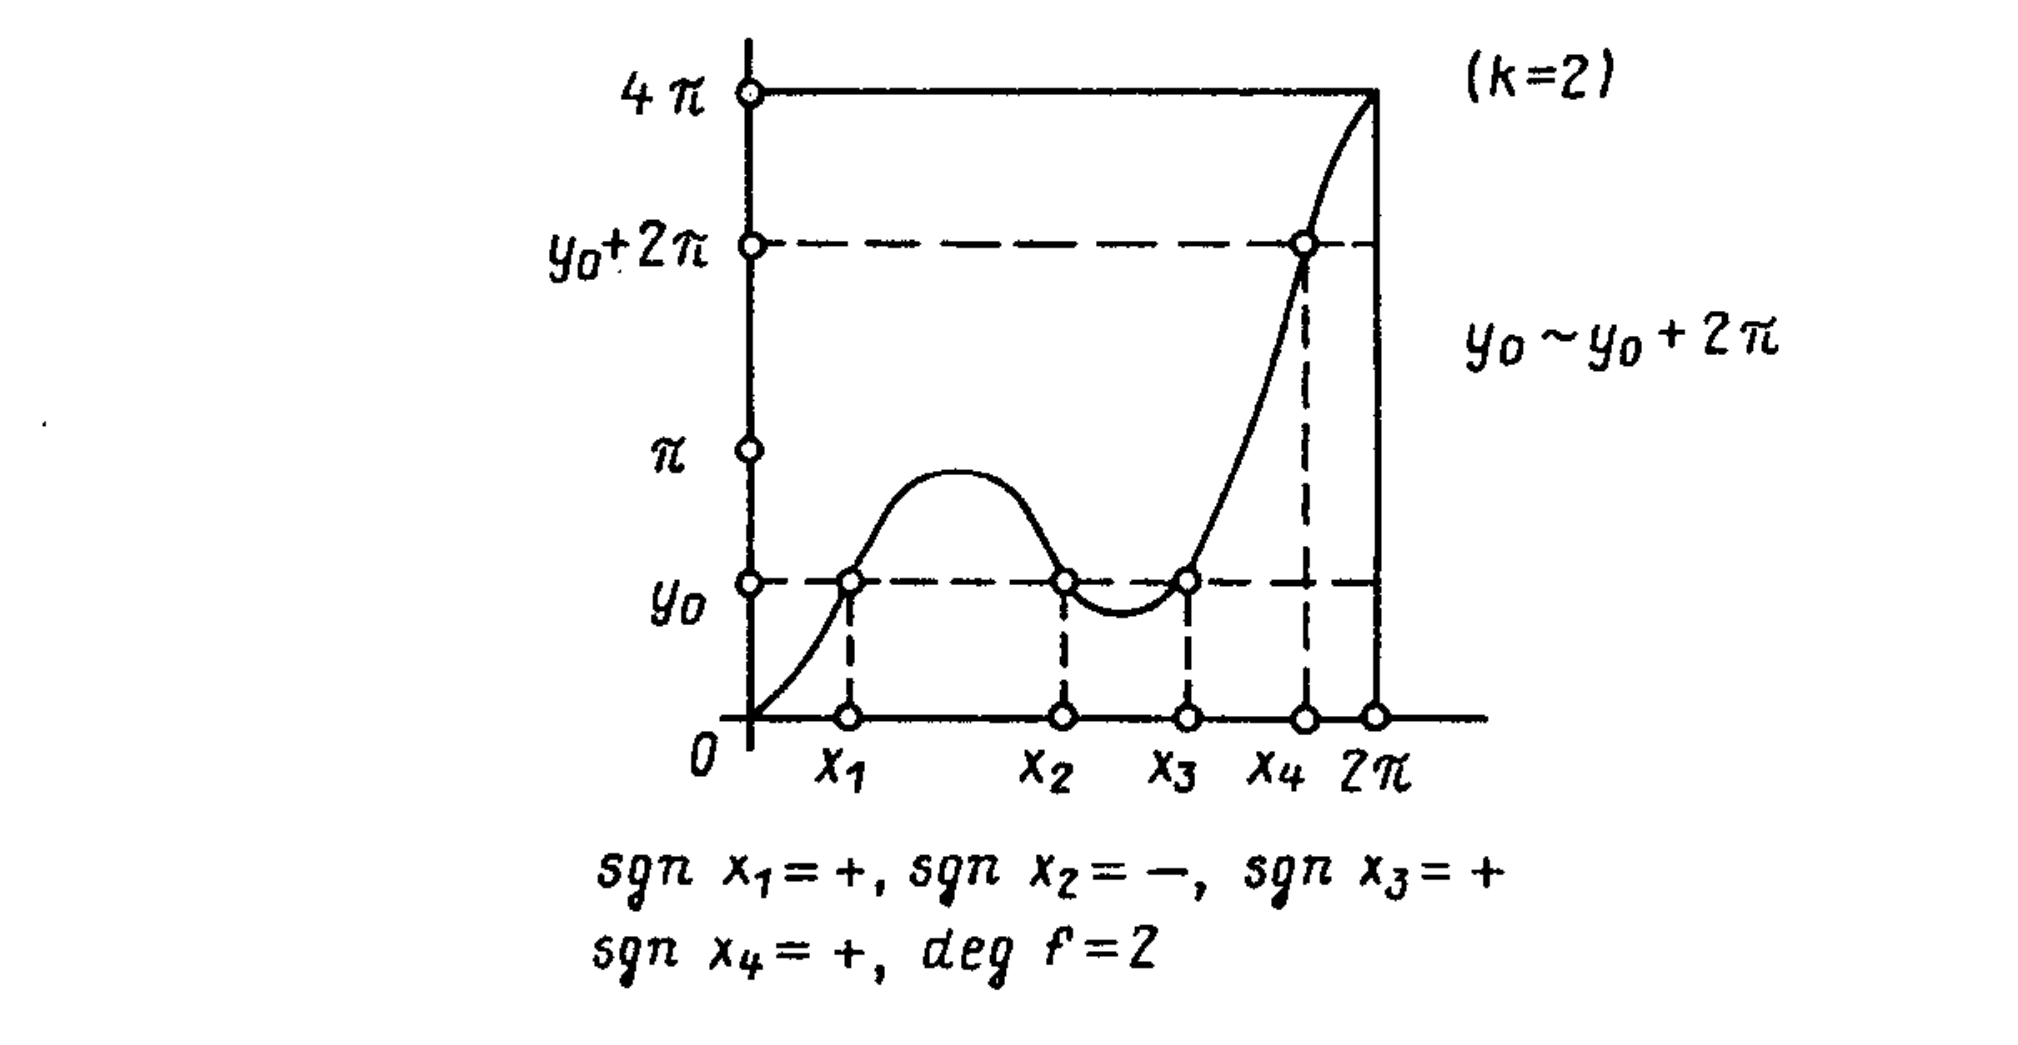
\includegraphics[width=0.72\textwidth]{figures/fig4_17.png}
  \figtitle{4.17}{把圆周映到圆周的映射的度：$y_0$ 与 $y_0+2\pi$ 等同，四个原像点符号依次为 $+,-,+,+$，度和为 $2$。}
\end{figure}

\para{b)} 开流形之间的\emph{真映射}（proper map）$f:M^n\to N^n$，即任一紧集的原像仍为紧集的映射。此时度在也构成真映射的同伦 $F:M^n\times I\to N^n$ 之下不变。注意：若 $\omega$ 是 $N^n$ 上的 $n$-形式，则有公式
\begin{equation}
  \int_{M^n}f^*\omega=(\deg f)\int_{N^n}\omega. \tag{3.2}
\end{equation}

\para{c)} 流形 $M^n$ 上向量场 $\eta(x)$ 的孤立奇点 $x_0$：$\eta(x_0)=0$。在以 $x_0$ 为心、半径 $\eps$ 充分小的球面 $S^{n-1}_\eps$（由 $|x-x_0|=\eps$ 定义）上，向量场 $\eta(x)$ 不为零，于是下列 Gauss 映射有定义：
\[
  \frac{\eta(x)}{|\eta(x)|}:S^{n-1}_\eps\to S^{n-1}.
\]
此映射的度称为奇点 $x_0$ 的\emph{指标}（index）。若奇点非退化，即
\[
  \det\left(\frac{\partial\eta^i}{\partial x^j}\right)\Big|_{x_0}\ne0,
\]
则奇点的指标等于 $\sgn\det(\partial\eta^i/\partial x^j)|_{x_0}$。（图 4.18 展示二维流形上向量场孤立非退化奇点的可能类型。）

% [原文 p.206]
对闭流形 $M^n$ 上的向量场，各奇点指标之和等于 Euler 示性数 $\chi(M^n)$（Poincaré、Hopf）。
\begin{figure}[htbp]
  \centering
  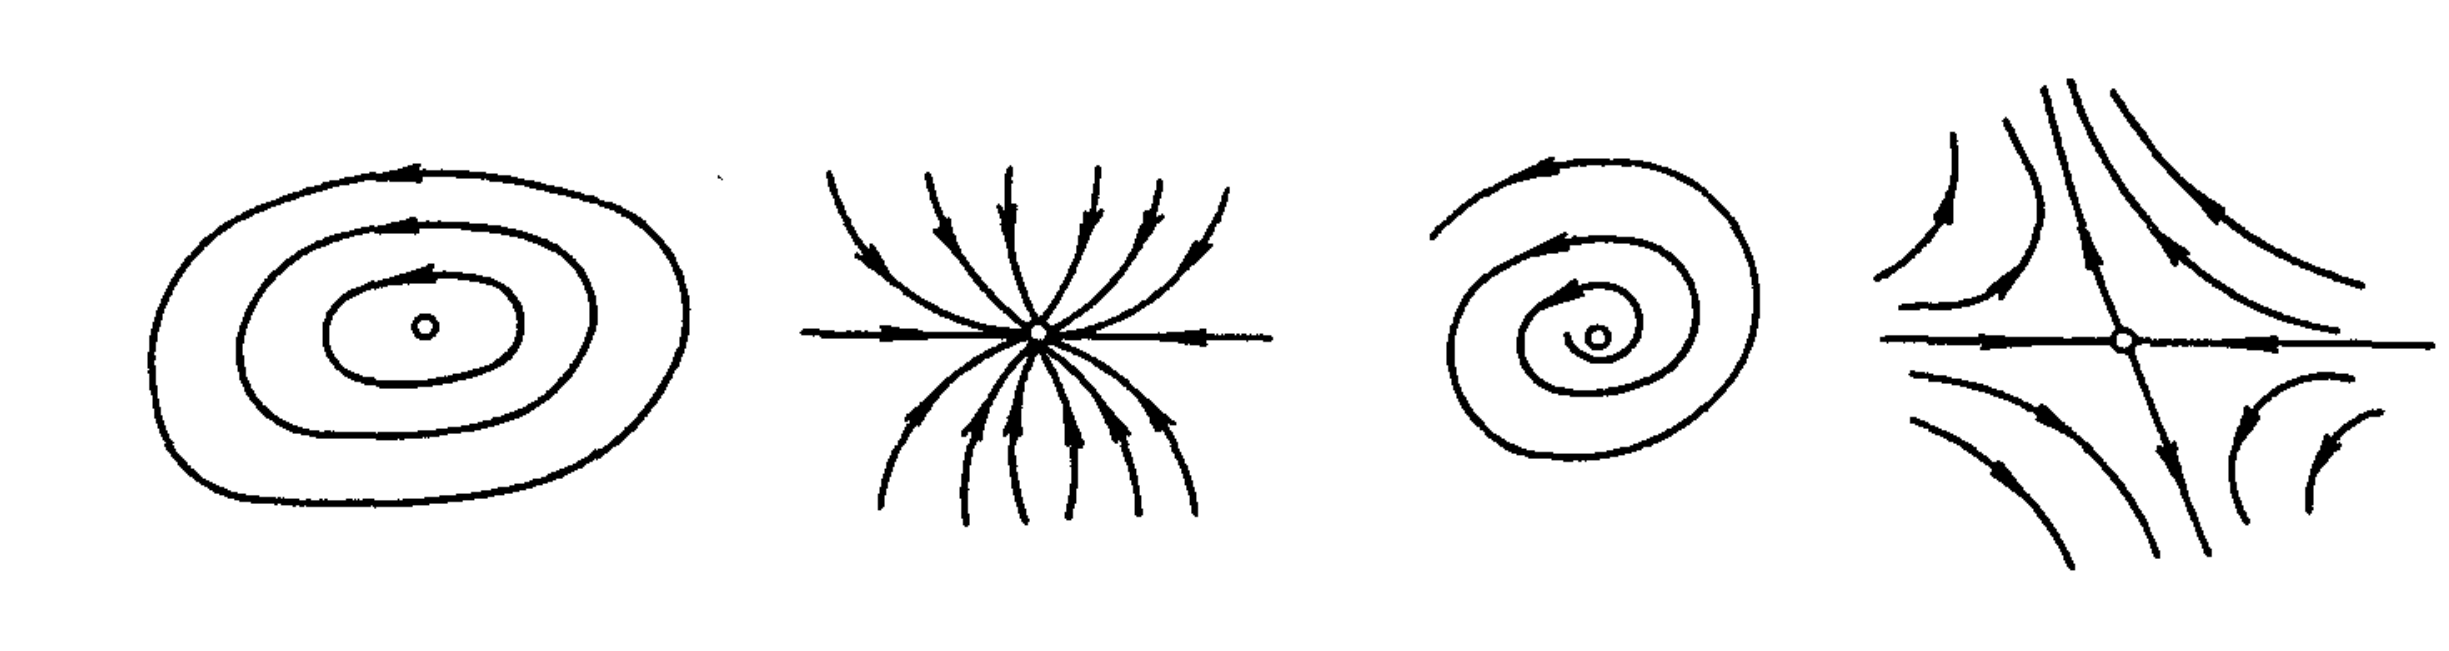
\includegraphics[width=0.90\textwidth]{figures/fig4_18.png}
  \figtitle{4.18}{二维流形上向量场孤立非退化奇点的类型：中心、源、螺线焦点与鞍点。}
\end{figure}

对不可定向流形，映射的度只模 $2$ 定义。如前所述，对连通流形，度与点 $y\in N^n$ 的选取无关。映射 $f:M^n\to N^n$ 的度的同伦不变性可这样看出：设 $F:M^n\times I\to N^n$ 是 $f$ 的任一同伦（$F(x,0)=f(x)$），取与 $y$ 任意接近的点 $\tilde y$，使得在 $F^{-1}(\tilde y)$ 的每一点处 $F$ 的秩为 $n$，如图 4.19 中 $M^n=N^n=S^1$ 的情形所示。该图中，$F$ 限制在柱面底与顶上的度相等是一目了然的，一般情形类似。
\begin{figure}[htbp]
  \centering
  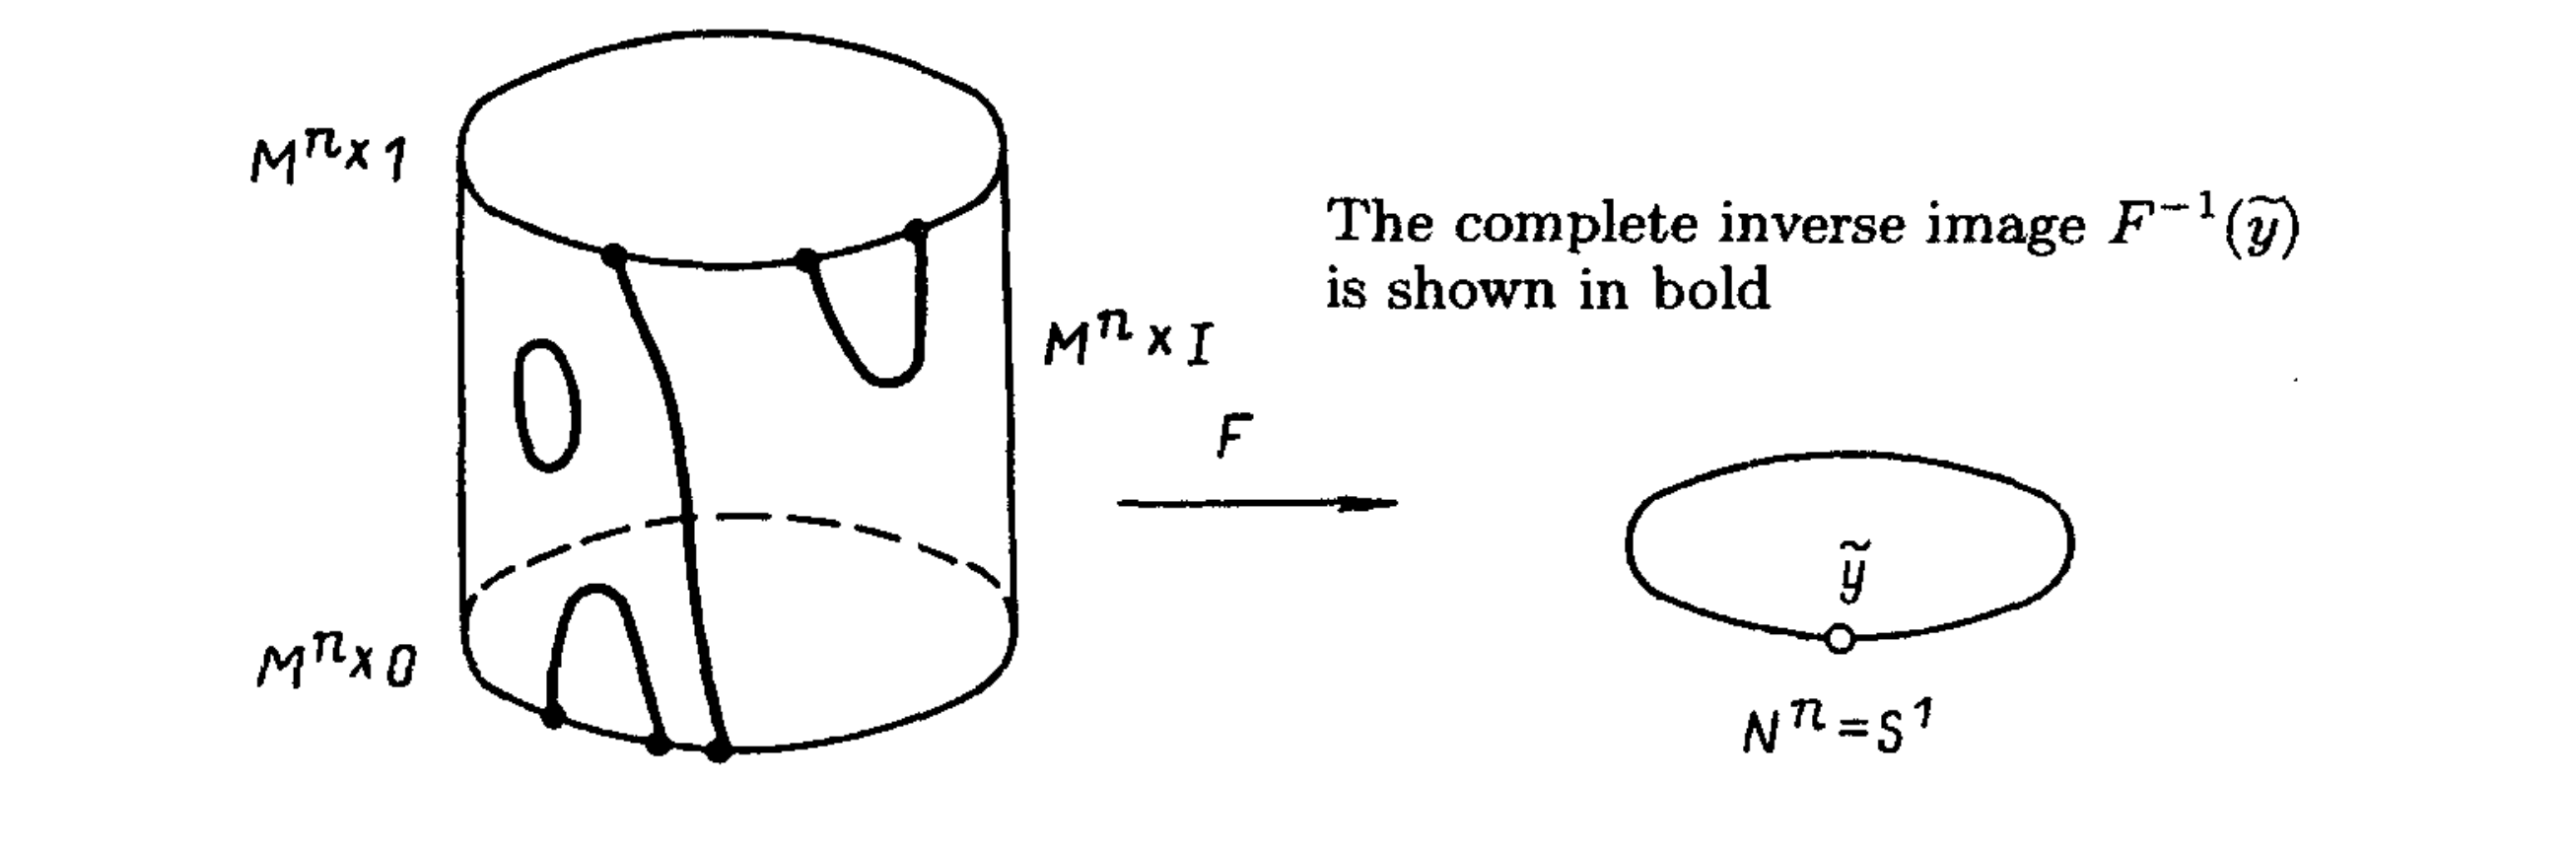
\includegraphics[width=0.86\textwidth]{figures/fig4_19.png}
  \figtitle{4.19}{度的同伦不变性：柱面 $M^n\times I$ 上的同伦 $F$，粗线为其完全原像 $F^{-1}(\tilde y)$。}
\end{figure}

Hopf 定理（20 世纪 20 年代末）断言：对闭流形 $M^n$，每个映射 $M^n\to S^n$ 在同伦意义下由它的度完全决定；因此度是这类映射的完全同伦不变量。Hopf 原来的论证沿着上述「度的同伦不变性」证明梗概进行，只是他用了 PL 流形，即流形的适当三角剖分。在更一般的情形——PL 流形之间的单纯（即 PL）映射 $f:M^{n+k}\to N^n$——$N^n$ 中维数最大的单形 $\sigma^n$ 的内部的完全原像将具有形式
\begin{equation}
  f^{-1}(\operatorname{Int}\sigma^n)=\operatorname{Int}\hat\sigma^n\times W^k, \tag{3.3}
\end{equation}
% [原文 p.207]
其中 $\hat\sigma^n$ 是 $M^{n+k}$ 的某个单形，$W^k$ 是子流形。循 Hopf 的想法，自然要利用这样的完全原像来寻找映射 $f$ 的不变量。
考虑球面之间的映射：
\[
  f:S^{n+k}\to S^n.
\]
回到一般位置点的用法，考虑两个不同点 $y_1,y_2\in S^n$ 的完全原像；它们将是子流形
\[
  W^k_i=f^{-1}(y_i),\qquad y_i\in S^n,\ i=1,2,
\]
\[
  W^k_1,W^k_2\subset S^{n+k}.
\]
当 $n$ 为偶数、$k=n-1$ 时，这两个子流形可在 $S^{n+k}=S^{2n-1}$ 中相链（linked），其\emph{环绕系数}（linking coefficient）为 $\{W^{n-1}_1,W^{n-1}_2\}$（环绕系数的定义见第 1 章）。对奇数 $n$，环绕系数 $\{W^{n-1}_1,W^{n-1}_2\}$ 为零。对偶数 $n$（即我们所考虑的情形），环绕系数与正则点对 $y_1,y_2\in S^n$ 的选取无关，且在 $f$ 的同伦下不变；它称为 $f$ 的\emph{Hopf 不变量}（Hopf invariant）：
\begin{align}
  h(f)&=\{W^{n-1}_1,W^{n-1}_2\},\qquad n=2q,\notag\\
  f&:S^{4q-1}\to S^{2q}. \tag{3.4}
\end{align}
Hopf 不变量决定了\emph{Hopf 同态}
\[
  \pi_{4q-1}(S^{2q})\to\Z,\qquad f\mapsto h(f),
\]
由此可知群 $\pi_{4q-1}(S^{2q})$ 无限。后来（20 世纪 50 年代初）Serre 证明其余所有 $\pi_j(S^n)$ 都有限；如前面（第 3 章 \S7）所见，这里所用的方法已远远超出纯粹几何的范围。
从 PL 映射转向光滑映射，就得到用点的完全原像研究球面同伦群的标准方法（Pontryagin，20 世纪 30 年代末）。在此方法中要利用这样的事实：映射 $f:S^{n+k}\to S^n$ 下正则点 $y\in S^n$ 的原像 $W^k=f^{-1}(y)$ 是\emph{标架流形}（framed manifold），即带有一个由 $f$ 决定的非退化 $n$-标架场 $\nu_n(x)$ 的流形，做法如下：设 $\phi_1,\dots,\phi_n$ 是 $y$ 的某个充分小邻域 $U$ 中的局部坐标，$y$ 为原点，且它们（相对 $S^n$ 上的标准局部坐标）的梯度线性无关；则完全原像 $W^k=f^{-1}(y)$ 由 $n$ 个方程 $\tilde\phi_1=0,\dots,\tilde\phi_n=0$ 给出，其中 $\tilde\phi_i$ 是 $\phi_i$ 到 $f^{-1}(U)$ 的提升。
% [原文 p.208]
梯度 $\operatorname{grad}\tilde\phi_i$ 在 $W^k$ 上线性无关，从而决定 $W^k$ 上的一个 $n$-标架场。
类似地，给定同伦 $F:S^{n+k}\times I\to S^n$，正则点 $y\in S^n$ 的完全原像 $F^{-1}(y)$ 是带边流形 $V^{k+1}\subset S^{n+k}\times I$（其边界分成两个不相交部分，一部分在柱面 $S^{n+k}\times I$ 的底上，另一部分在顶上），它按与上面大致相同的方式配有一个法向（相对于某个 Riemann 度量）向量 $n$-标架场 $\nu_n(x)$，该标架场在 $V^{k+1}$ 的边界上落在 $S^{n+k}\times\{a\}$ 或 $S^{n+k}\times\{b\}$ 中。（注意可以假定 $V^{k+1}$ 横截地接近 $S^{n+k}\times I$ 的顶与底。）对 $(V^{k+1},\nu_n)\subset S^{n+k}\times I$ 称为\emph{带边标架流形}（或\emph{标架配边}）。两个标架流形 $(W^k_1,\nu^{(1)}_n)$、$(W^k_2,\nu^{(2)}_n)$ 称为\emph{等价的}，若存在标架配边 $(V^{k+1},\nu_n)$（$V^{k+1}\subset S^{n+k}\times I$），其各边界分支恰为给定的标架流形。实现这种等价的流形可称为\emph{标架配边}（framed bordism，或 framed cobordism）。不难证明：闭标架流形的等价类与群 $\pi_{n+k}(S^n)$ 的元素自然一一对应。
在继续之前，我们指出：当 $k<n-1$ 时群 $\pi_{n+k}(S^n)$ 称为\emph{稳定的}（stable），因为对这些 $k$ 它们与 $n$ 无关；这由悬挂同构
\[
  \Sigma:\pi_{n+k}(S^n)\to\pi_{n+k+1}(S^{n+1}),\qquad k<n-1
\]
立即看出。
更一般地，对任意 CW 复形 $K$，悬挂构造在同调中总给出同构（见第 3 章 \S3）；而当 $K$ 是 $(n-1)$-连通的（即当 $j\le n-1$ 时 $\pi_j(K)=0$）且 $k<n-1$ 时，给出同构
\[
  \Sigma:\pi_{n+k}(K)\xrightarrow{\ \cong\ }\pi_{n+k+1}(\Sigma K).
\]
（这是 Freudenthal 在 20 世纪 30 年代末证明的；他也是第一个算出群 $\pi_{n+1}(S^n)$ 的人。）

关于标架流形的以下事实不难建立：
\para{1.} 维数 $k>0$ 的每个标架流形 $(W^k,\nu_n)$ 都等价于一个连通的标架流形。（图 4.20 说明如何构造带边标架流形 $(V^{k+1},\nu_n)$，其边界 $\partial V^{k+1}=W^k_1\cup W^k_*\cup W^k_2$；该流形实现不交并 $(W^k_1\cup W^k_2,\ \nu_n|_{W^k_1\cup W^k_2})$ 与连通标架流形 $(W^k_*,\ \nu_n|_{W^k_*})$ 之间的等价。）
\para{2.} 当 $k=1$ 时，标架流形唯一的稳定不变量是其标架场的同伦类，后者由映射 $\nu_n:S^1\to SO_n$ 给出。由于 $n\ge3$ 时 $\pi_1(SO_n)\cong\Z/2$，由此得 $n\ge3$ 时 $\pi_{n+1}(S^n)\cong\Z/2$。
\para{3.} 当 $k=2$ 时，标架流形的每个等价类 $(W^2,\nu_n)$ 仍只有一个稳定不变量，但它的构造要复杂一些。设 $n>4$。由上面的断言 1，不妨设 $W^2\subset\R^{n+2}$（或 $W^2\subset S^{n+2}$）是带法向场 $\nu_n(x)$ 的连通曲面（比如亏格为 $g$）。每个类 $z\in H_1(W^2;\Z/2)$ 都可由 $W^2\subset\R^{n+2}$ 中一条简单（即嵌入的）圆周 $C\cong S^1$ 代表。

% [原文 p.209]
以 $n(x)$ 记 $C$ 在 $W^2$ 中的法向量场，于是得到 $C$ 在 $\R^{n+2}$ 中的法标架场 $\nu_{n+1}(x)=(n(x),\nu_n(x))$。由上面的断言 2，标架流形 $(C,\nu_{n+1}(x))$ 有唯一的不变量，记作 $\Phi(z)\in\Z/2$，称为\emph{Arf 函数}。有如下「Arf 恒等式」：
\begin{equation}
  \Phi(z_1+z_2)=\Phi(z_1)+\Phi(z_2)+z_1\circ z_2\pmod 2, \tag{3.5}
\end{equation}
其中 $z_1\circ z_2$ 是闭链 $z_1$ 与 $z_2$ 的相交指数。用任意典范闭链基 $z_1,\dots,z_g,w_1,\dots,w_g$（即满足
\[
  z_i\circ z_j=w_i\circ w_j=0,\qquad z_i\circ w_j=\delta_{ij}
\]
的基），完全的 Arf 不变量定义为
\begin{equation}
  \Phi=\sum_{i=1}^g\Phi(z_i)\Phi(w_i),\qquad \Phi\in\Z/2. \tag{3.6}
\end{equation}
（它与（典范）基的选取无关。）可以证明：当 $n\ge4$ 时，量 $\Phi$ 是标架流形 $(W^2,\nu_n)$ 的唯一稳定不变量；由此推出 $n\ge4$ 时 $\pi_{n+2}(S^n)\cong\Z/2$（Pontryagin，20 世纪 40 年代末）。
\begin{figure}[htbp]
  \centering
  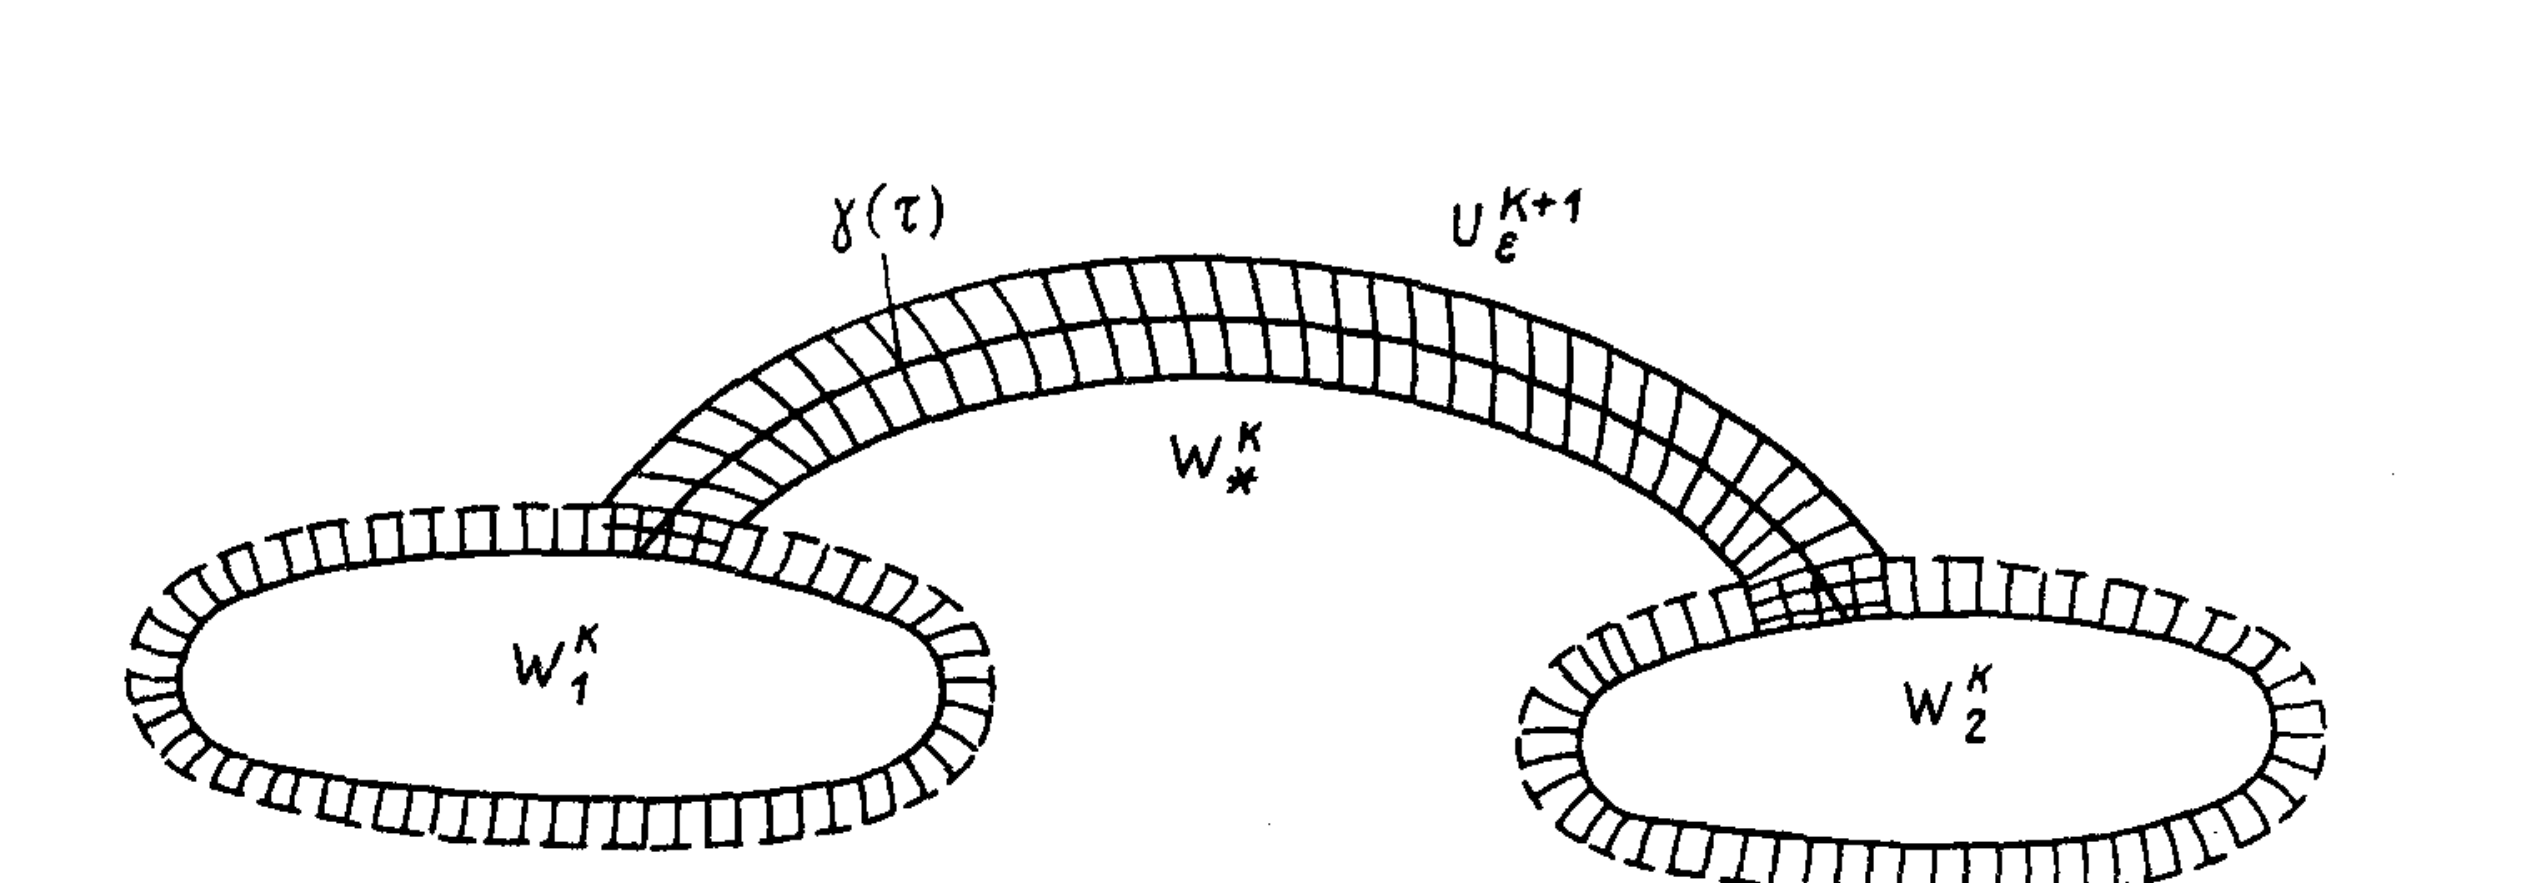
\includegraphics[width=0.86\textwidth]{figures/fig4_20.png}
  \figtitle{4.20}{把两个标架流形 $W^k_1$、$W^k_2$ 连接成连通标架流形 $W^k_*$ 的带边标架流形 $U^{k+1}_\eps$，$\gamma(\tau)$ 为其上的一条积分曲线。}
\end{figure}

\para{4.} 有一个复杂的理论（Rohlin 在 20 世纪 50 年代初创立），导致群 $\pi_{n+3}(S^n)$ 的确定。作为第一步（非平凡的一步），要证明每个非平凡的标架流形 $(W^3,\nu_n)$ 都配边于标架球面 $S^3\subset\R^{n+3}$，且其中 $S^3$ 在 $\R^{n+3}$ 中处于标准位置（因为在稳定范围内，$S^3$ 在 $\R^{n+3}$ 中的每种位置都等价于标准位置）。接着证明：在 $S^3\subset\R^{n+3}$ 上定义标架时的自由度决定一个同态（实际上是满同态）
\begin{equation}
  J:\pi_3(SO_n)\to\pi_{n+3}(S^n). \tag{3.7}
\end{equation}
由于 $n>4$ 时 $\pi_3(SO_n)\cong\Z$，由此可知稳定群 $\pi_{n+3}(S^n)$ 是循环群。进一步的分析表明
\[
  \pi_{n+3}(S^n)\cong\Z/24\quad(n>4),\qquad
  \pi_7(S^4)\cong\Z\oplus\Z/12,\qquad
  \pi_6(S^3)\cong\Z/12.
\]
% [原文 p.210]
% [Tutor Note: 原书 p.210 首行把 $\pi_{n+3}(S^n)$ 排作 $\pi_{n+3}(S_n)$（$S$ 带下标 $n$），按上下文与 p.209 的记法，疑为笔误，这里写作 $S^n$。]
这些结果与 Rohlin 定理密切相关。Rohlin 定理断言：对闭流形 $M^4$，若 $M^4\setminus\{x_0\}$ 可平行化，则第一 Pontryagin 类 $p_1(M^4)$ 可被 $48$ 整除。（回想示性类是整上同调群的元素。）
作为 (3.7) 的推广，有：标架 $k$-球面 $(S^k,\nu_n)$ 的等价类在 $\pi_{n+k}(S^n)$ 中决定「Whitehead 同态」（见第 3 章 \S8）
\[
  J:\pi_k(SO_n)\to\pi_{n+k}(S^n)
\]
的像。
已知这个像是有限循环群；其阶（一个重要的量）在 $k=4s-1$ 时可用 Bernoulli 数表示。（Milnor 与 Kervaire 在 20 世纪 50 年代末给出该阶的下界，Adams 在 60 年代中期给出上界。）\hfill$\square$

这些结果表明了用几何方法研究球面同伦群所能达到的极限；此问题的进一步进展需要大量使用同伦论方法（见第 3 章 \S7）。

配边与上配边理论可视为上述几何想法的自然发展，它是一座通往代数技术的桥梁，用以解决关于光滑流形的问题。经典的\emph{配边群}（bordism group，或 cobordism group）定义如下：同维数 $k$ 的两个光滑闭流形 $W^k_1$、$W^k_2$ 称为\emph{等价的}（或\emph{配边的}），若它们的和（即不交并）微分同胚于某个紧光滑流形 $N^{k+1}$ 的边界：
\[
  W^k_1\cup W^k_2\cong\partial N^{k+1}.
\]
对每个 $k\ge0$，闭 $k$-流形的等价（或配边）类按由流形求和运算显然定义的操作构成群 $\Omega^O_k$。直和
\begin{equation}
  \Omega^O_*=\sum_{k\ge0}\Omega^O_k \tag{3.8}
\end{equation}
于是构成分次环\footnote{配边环 $\Omega^O_*$ 另有一个标准记号 $\Im_*$。}，即\emph{经典配边环}，其乘法运算由流形的直积确定。它实际上是 $\Z/2$ 上的代数。
\para{例.} 1. $\Omega^O_0\cong\Z/2$（标量）。2. $\Omega^O_1=0$。

% [原文 p.211]
3. $\Omega^O_2\cong\Z/2$。（这由闭曲面的分类定理推出。注意 $\RP^2$ 代表非零元素，即 $\RP^2$ 不是任何紧三维流形的边界。由于 $\chi(\RP^2)=-1$，这可由以下一般事实推出：若闭流形是边界，即 $M^n=\partial W^{n+1}$，则它的 Euler--Poincaré 示性数为偶数。这又是等式
\[
  \chi(W^{n+1}\cup_{M^n}W^{n+1})=2\chi(W^{n+1})-\chi(M^n)
\]
的推论，其中 $W^{n+1}\cup_{M^n}W^{n+1}$ 是 $W^{n+1}$ 的「倍」（取 $W^{n+1}$ 的两份并把边界等同而得），同时用到任何奇维闭流形的 Euler--Poincaré 示性数为零这一事实。）
3. $\Omega^O_3=0$（Rohlin，20 世纪 50 年代初）。\hfill$\square$
% [Tutor Note: 原书 p.211 的例子编号有重复：$\Omega^O_2$ 与 $\Omega^O_3$ 两条都标作 3.，后者按顺序应为 4.。此处照原书排印。]

若只考虑可定向流形，类似地得到\emph{可定向配边群} $\Omega^{SO}_k$ 与\emph{可定向配边环}
\[
  \Omega^{SO}_*=\sum_{k\ge0}\Omega^{SO}_k.
\]
\para{例.} 1. $\Omega^{SO}_0\cong\Z$（标量）。
2. $\Omega^{SO}_1=0=\Omega^{SO}_2$（显然）。
3. $\Omega^{SO}_3=0$（Rohlin，20 世纪 50 年代初）。
4. $\Omega^{SO}_4\cong\Z$（Rohlin 与 Thom，均在 20 世纪 50 年代初）。注意配边类 $[\CP^2]$ 生成 $\Omega^{SO}_4$。\hfill$\square$

若闭流形 $M^n$ 是边界，即在配边群 $\Omega^O_n$ 中代表零，则它的所有「Stiefel--Whitney 数」（见下文）都为零。20 世纪 40 年代末 Pontryagin 建立了以下基本事实：若闭的 $4k$ 维流形 $M^{4k}$ 是可定向流形的边界，则此外它的「Pontryagin 数」也全为零。$M^n$ 的\emph{Stiefel--Whitney 示性数}是 $\Z/2$ 上关于 Stiefel--Whitney 示性类的 $n$ 次齐次多项式在基本类 $[M^n]$ 上取的值。（为得到 $M^{4k}$ 的\emph{Pontryagin 示性数}，要在 Pontryagin 示性类中取 $\Z$ 上 $k$ 次齐次多项式并求值。）
计算配边群的主要方法基于它们与同伦论的联系；下面描述这种联系。

\begin{definition*}{3.1}
向量丛 $\eta$（或任何以 $\R^n$ 为纤维的纤维丛）的\emph{Thom 空间} $T_\eta$ 是商空间 $E/\Delta E$，其中 $\Delta E$ 由各纤维中长度 $\ge1$ 的向量组成的子空间。（若 $\eta$ 的底 $B$ 是紧空间，也可取全空间 $E$ 的一点紧化，因为所得空间同伦等价于 Thom 空间 $T_\eta$。）
\end{definition*}
% [原文 p.212]
对每个 $j\ge0$ 都有自然同构，即\emph{Thom 同构}（若丛不可定向，则在模 $2$ 上同调中成立）：
\begin{equation}
\begin{gathered}
  \phi:H^j(B)\to H^{j+n}(T_\eta),\qquad j\ge0,\\
  \phi(z)=z\cdot u_n,\qquad u_n=\phi(1),
\end{gathered}\tag{3.9}
\end{equation}
其中 $\phi(1)$ 是 $T_\eta$ 的上同调类，它在各纤维上取值 $1$，称为\emph{Thom 类}。有下面的 Thom 公式（20 世纪 50 年代初），它把向量丛 $\eta$ 的 Stiefel--Whitney 示性类 $w_j\in H^j(B;\Z/2)$ 与 Steenrod 平方 $Sq^j$ 联系起来：
\begin{equation}
  w_j(\eta)=\phi^{-1}Sq^j\phi(1). \tag{3.10}
\end{equation}
把它应用于光滑闭流形 $M^n$ 的切丛 $\tau(M^n)$，就得到 $M^n$ 的 Stiefel--Whitney 类 $w_j(M^n)$ 的同伦不变性的一个证明。利用切丛 $\tau(M^n)$ 同构于对角子流形 $\Delta\subset M^n\times M^n$ 的法丛这一事实，结合 Thom 公式 (3.10)，可以把类 $w_j(M^n)$ 用作用在上同调环 $H^*(M^n;\Z/2)$ 上的 Steenrod 平方 $Sq^i$ 显式表示出来（Wu 公式，20 世纪 50 年代初）。为得到 Wu 公式，要对每个 $i=1,\dots,[n/2]$ 在群 $H^{n-i}(M^n;\Z/2)$ 上解方程
\begin{equation}
  Sq^i(z)=z\cdot\kappa_i, \tag{3.11}
\end{equation}
以求出未知的 $\kappa_i$（对一切 $z\in H^{n-i}(M^n;\Z/2)$）。我们指出，方程 (3.11) 有解，因为任何同态 $H^{n-i}(M^n;\Z/2)\to\Z/2$（特别地，同态
\[
  Sq^i:H^{n-i}(M^n;\Z/2)\to H^n(M^n;\Z/2)\cong\Z/2
\]
）都可经 Poincaré 对偶、通过用某个单一的 $i$ 维类乘 $H^{n-i}$ 中的元素而得到。Wu 公式的形式如下：
\begin{equation}
\begin{gathered}
  Sq(w)=\kappa,\\
  w=1+w_1+\cdots+w_n,\\
  \kappa=1+\kappa_1+\cdots+\kappa_{[n/2]},\\
  Sq=1+Sq_1+Sq_2+\cdots.
\end{gathered}\tag{3.12}
\end{equation}
% [Tutor Note: 原书此处把总 Steenrod 平方的分解印作下标形式 $Sq=1+Sq_1+Sq_2+\cdots$，与全书其余地方的上标记法 $Sq=1+Sq^1+Sq^2+\cdots$ 不一致；按本书「照原书排印、以批注说明」的惯例保留原样，阅读时宜按 $Sq^i$ 理解。]
这些公式给出例如下述结果：所有可定向三维流形都是可平行化的。
% [原文 p.213]
若流形 $M^n$ 几乎可平行化（almost parallelizable），即挖去一点后的 $M^n\setminus\{x_0\}$ 可平行化，则 $w_i=0$（$i<n$）。由此并结合 (3.12) 可推出：若 $n=4k$，则在 $H^{2k}(M^n;\Z/2)$ 中每个平方都为零，即 $z^2\equiv0\pmod2$。这意味着对每个
\[
  z\in H^{2k}(M^{4k};\Z)/(\text{挠部分}),
\]
纯量平方 $(z^2,[M^{4k}])=\langle z,z\rangle$ 都是偶数。
% [Tutor Note: 「偶幺模二次型的符号差被 8 整除」是二次型理论中的经典引理，原书直接引用而未证明；这里的「幺模」指相交形式在 $H^{2k}(M^{4k};\Z)/\text{Torsion}$ 上非退化。]
由于二次型 $\langle z,z\rangle$ 是偶的且幺模，于是符号差 $\tau(M^{4k})$ 可被 $8$ 整除。\emph{符号差} $\tau(M^{4k})$ 定义为元素 $x,y\in H_{2k}(M^{4k};\Z)$ 的相交指数所给出的（对角化的）二次型 $\langle x,y\rangle$ 中正平方项与负平方项个数之差（等价地，由 $\langle x,y\rangle=(xy,[M^{4k}])$ 给出，其中 $x=Dx$，$y=Dy$），不过该二次型只对闭流形才非退化。可以证明，对闭流形，符号差在配边下不变：若 $M^{4k}=\partial W^{4k+1}$，其中 $W^{4k+1}$ 是某个可定向带边流形，则 $\tau(M^{4k})=0$。（为证明这一点，先注意：若 $M^{4k}$ 中两个 $2k$-闭链在 $W^{4k+1}$ 中零同调，则它们的相交指数为零，于是 $\langle\,,\rangle$ 在 $\operatorname{Im}i^*$ 上为零，其中 $i^*$ 是包含同态 $H^{2k}(W^{4k+1};\Q)\to H^{2k}(M^{4k};\Q)$。再证明 $\operatorname{Im}i^*\subset H^{2k}(M^{4k};\Q)$ 的维数恰为 $H^{2k}(M^{4k};\Q)$ 的维数的一半，即得所需结论。）由这一事实可得重要推论；例如群 $\Omega^{SO}_4$ 同构于 $\Z$，由 $[\CP^2]$ 生成。在 §1 中我们看到 $\CP^2$ 的第一 Pontryagin 类 $p_1$ 满足
\[
  (1+p_1)=(1+u^2)^3=1+3u^2\in H^*(\CP^2;\Z),
\]
其中 $u$ 是 $H^2(\CP^2;\Z)\cong\Z$ 的生成元。由此 $p_1(\CP^2)=3$。又 $\tau(\CP^2)=1$（这可直接由 $H^*(\CP^2;\Q)$ 的结构得到），且 $[\CP^2]$ 生成 $\Omega^{SO}_4$，故对每个可定向闭四维流形 $M^4$ 都有
\begin{equation}
  \tau(M^4)=\frac13p_1, \tag{3.13}
\end{equation}
因为 $3\tau(M^4)-p_1$ 是 $\Omega^{SO}_4\cong\Z$ 上的恒为零的线性形式。（这一结果属于 Rohlin 与 Thom，20 世纪 50 年代初。）把公式 (3.13) 推广到更高维，需要计算群 $\Omega^{SO}_j\otimes\Q$；这一问题将在后文讨论。
带边流形 $M^{4k}$ 的符号差 $\tau(M^{4k})$ 具有\emph{可加性}：若 $M^{4k}_1$、$M^{4k}_2$ 是两个带边流形，$V_1,V_2\cong V$ 分别是它们边界中微分同胚的连通分支，则把 $V_1$ 与 $V_2$ 等同所得的流形满足（Rohlin 与 Novikov，20 世纪 60 年代末）
\begin{equation}
  \tau(M^{4k}_1\cup M^{4k}_2)=\tau(M^{4k}_1)+\tau(M^{4k}_2). \tag{3.14}
\end{equation}
我们指出，偶维流形 $M^{2k}$ 的 Poincaré--Euler 示性数也具有这种可加性，而其它示性类则没有。
% [原文 p.214]
对任意群 $G\subset O_m$，以 $BG$ 为底、纤维为 $\R^m$ 的万有向量丛的 Thom 空间记作 $M(G)$。更一般地，任一表示 $\rho:G\to O_m$（不必一一）都决定一个 Thom 空间；例如二重覆叠
\[
  \rho:Spin_m\to SO_m
\]
决定 Thom 空间 $M(Spin_m)$。若 $G\subset SO_m$，则称 $M(G)$ 为\emph{可定向 Thom 空间}。在 $G=\{1\}\subset SO_m$ 的情形得到 $m$-球面：$M(G)\cong S^m$。由 (3.9) 有下述 Thom 同构：
\[
\begin{gathered}
  \text{a)}\quad \phi:H^j(BG;\Z)\to H^{m+j}(M(G);\Z),\qquad G\subset SO_m,\\
  \phi(z)=z\cdot u_m,\qquad u_m=\phi(1);
\end{gathered}
\]
\[
\begin{gathered}
  \text{b)}\quad \phi:H^j(BG;\Z/2)\to H^{m+j}(M(G);\Z/2),\qquad G\subset O_m,\\
  \phi(z)=z\cdot u_m,\qquad u_m=\phi(1).
\end{gathered}
\]
经典的配边论（如我们所见）集中于 $G=O_m$ 或 $SO_m$ 的情形。该理论的进一步发展基于以下事实（由 Thom 建立）：
\para{(i)} 元素 $z\in H_{n-m}(M^n;\Z/2)$ 可由闭子流形 $W^{n-m}\subset M^n$ 表示，当且仅当存在映射 $f:M^n\to M(O_m)$ 使
\[
  f^*(u_m)=Dz\in H^m(M^n;\Z/2),
\]
其中 $u_m=\phi(1)$ 是 Thom 空间 $M(O_m)$ 的 Thom 类（见 (3.9)），$D$ 是 Poincaré 对偶同构。
\para{(ii)} 设 $M^n$ 可定向。元素 $z\in H_{n-m}(M^n;\Z)$ 可由可定向子流形 $W^{n-m}\subset M^n$ 表示，当且仅当存在映射 $f:M^n\to M(SO_m)$ 使
\[
  f^*(u_m)=Dz\in H^m(M^n;\Z).
\]
\para{(iii)} 配边群 $\Omega^O_k$、$\Omega^{SO}_k$ 自然同构于 $M(O_m)$、$M(SO_m)$ 的相应「稳定」同伦群：
\begin{equation}
\begin{gathered}
  \Omega^O_k\cong\pi_{m+k}(M(O_m)),\qquad k<m-1,\\
  \Omega^{SO}_k\cong\pi_{m+k}(M(SO_m)),\qquad k<m-1
\end{gathered}\tag{3.15}
\end{equation}
（Thom，20 世纪 50 年代初）。
注意，若在 (3.15) 中把 $SO_m$ 换成平凡群 $\{1\}$，就得到 Pontryagin（20 世纪 30 年代末）建立的同构，它联系
\[
  \pi_{m+k}(M(\{1\}))=\pi_{m+k}(S^m)
\]
与标架流形的配边群 $\Omega^{fr}_k$，$k<m-1$。
% [原文 p.215]
上述陈述 (i)、(ii)、(iii) 是用「横截正则性定理」（或 $t$-正则性）建立的。该定理说：光滑流形之间的任一映射 $g:M^n\to X^q$ 都可用在任意指定的子流形 $Y^{q-m}\subset X^q$ 上「$t$-正则」的映射 $f$ 任意逼近。（映射 $f$ 在 $Y^{q-m}$ 上是 $t$-正则的，是指：对完全原像 $f^{-1}(Y^{q-m})\subset M^n$ 的每一点 $y$，$M^n$ 在 $y$ 处的切空间（在切空间之间的诱导映射下）的像，连同 $Y^{q-m}$ 在 $f(y)$ 处的切空间，一起张成 $X^q$ 在 $f(y)$ 处的整个切空间。）这一条件保证完全原像 $f^{-1}(Y^{q-m})$ 是 $M^n$ 的维数为 $n-m$ 的光滑子流形：
\[
  f^{-1}(Y^{q-m})=N^{n-m}\subset M^n,
\]
而且限制映射 $N^{n-m}\to Y^{q-m}$ 自然延拓为相应法丛（纤维为 $\R^m$）之间的映射。
为得到闭链可由子流形表示（陈述 (i)、(ii)），取 $M(O_m)$（或 $M(SO_m)$）充当 $X^q$，取 $BO_m\subset M(O_m)$（或 $BSO\subset M(SO_m)$）充当 $Y^{q-m}$；表示闭链的子流形就是 $f^{-1}(BO_m)$（或 $f^{-1}(BSO_m)$）。为得到陈述 (iii)，取 $X^q=S^q$。

\begin{remark}{}
空间 $M(O_n)$ 与 $M(SO_n)$ 连同自然映射
\[
  M(O_n)\to M(O_{n+1}),\qquad M(SO_n)\to M(SO_{n+1})
\]
定义\emph{谱}（spectrum，即适当范畴中的对象），分别记作 $MO$ 与 $MSO$。谱 $MO$ 与 $MSO$ 的「同伦群」与上述「稳定」同伦群一致：
\[
\begin{gathered}
  \pi_kMO=\pi_{m+k}(M(O_m)),\qquad k<m-1,\\
  \pi_kMSO=\pi_{m+k}(M(SO_m)),\qquad k<m-1.
\end{gathered}
\]
谱 $MU$、$MSU$、$MSpin$ 与 $MSp$ 用类似方式定义。\hfill$\square$
\end{remark}

同伦群 $\pi_*(M(G))$（$G\subset O_m$）有一个自然的几何解释，如下所述。称子流形 $W^k\subset S^{m+k}$（或 $\R^{m+k}$）上的法丛 $\nu_m$ 配备 $G$-结构后为\emph{$G$-流形}。两个 $G$-流形 $W^m_1,W^m_2\subset S^{m+k}$ 称为\emph{$G$-配边的}，若存在与边界横截的 $G$-流形 $V^{m+1}\subset S^{m+k}\times I$，$I=[a,b]$，使
\[
  \partial V=W^m_1\cup W^m_2,
\]
\[
  W^m_1\subset S^{n+k}\times\{a\},\qquad W^m_2\subset S^{n+k}\times\{b\}
\]
（与前面引入的标架配边类似）。
% [Tutor Note: 原书 p.215 这几行把 $G$-流形与配边的上标排作 $m$（$W^m_1$、$V^{m+1}$），而按定义其维数应为 $k$；末式又印 $S^{n+k}$ 而上文用 $S^{m+k}$。此处照原书排印，疑为笔误。]

% CHUNK ch04f DONE
